%%%%%%%%%%%%%%%%%%%%%%%%%%%%%%%%%%%%%%%%%%%%%%%%%%%%%%%%%%%%%%%%%%%%%%
%%                     Perturbing Agent
%%%%%%%%%%%%%%%%%%%%%%%%%%%%%%%%%%%%%%%%%%%%%%%%%%%%%%%%%%%%%%%%%%%%%%

%\color{blue}

Biochemical networks can be affected by external influences. Those
influences can be well-defined physical perturbations, such as a the effect of a light
pulse or of a change in temperature; they can also be more complex and not
well-defined phenomena, for instance a biological process, an experimental
setup, or a mutation.  For these situations, SBGN provides the
\glyph{perturbing agent} glyph. We do not use the word \emph{perturbation} to avoid the misunderstanding with the influence that the \glyph{perturbing agent} has on the map. 

\begin{glyphDescription}

\glyphSboTerm SBO:0000405 ! perturbing agent

\glyphContainer A \glyph{perturbing agent} is represented by a modified hexagon
having two opposite concave faces, as illustrated in \fig{perturbation}.

\glyphLabel A \glyph{perturbing agent} is identified by a label placed in an
unbordered box containing a string of characters.  The characters can be
distributed on several lines to improve readability, although this is not
mandatory.  The label box must be attached to the center of the
\glyph{perturbing agent} container.  The label may spill outside of the container.

\glyphAux A \glyph{perturbing agent} does not carry any auxiliary unit. In particular, its existence being not subjected to any modulation by any other \glyph{interactor}, it does not require the state variable existence. \glyph{Perturbing agent} do not have location either. pH of lysosome and mitochondria are different perturbing agents. 

\end{glyphDescription}

\begin{figure}[H]
  \centering
  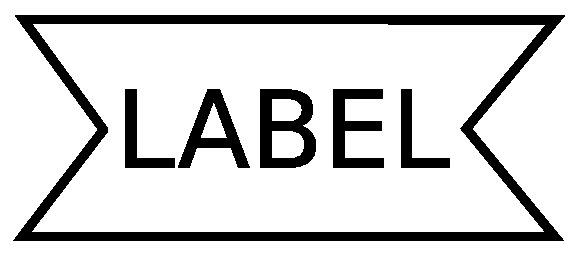
\includegraphics[scale = 0.3]{images/perturbation}
  \caption{The \ER glyph for \glyph{perturbing agent}.}
  \label{fig:perturbation}
\end{figure}

\begin{figure}[H]
  \centering
  \includegraphics[scale = 0.5]{examples/ex-perturbing}
  \caption{Example of a \glyph{perturbing agent} representing the depolarisation of a membrane, that stimulates (\sect{stimulation}) the existence (see \ref{sec:existence}) of an interactor.}
  \label{fig:ex-perturbing}
\end{figure}

\normalcolor
